% !TEX root = ../InterpolatingOTFR.tex

%%%%%%%%%%%%%%%%%%%%%%%%%%%%%%
%%%%%%%%%%%%%%%%%%%%%%%%%%%%%%
\section{Explicit geodesics}
\label{sec-explicit-geod}

In this section, we give an explicit description of the behavior of geodesics in three cases: for an ``inflating'' measure, for the transport of one Dirac measure to another, and finally for the transport of multiple couples of Dirac measures. In order to establish explicit geodesics, we will first exhibit an ansatz and then prove the existence of an optimality certificate as defined in \thref{certificate}.

%%%%%%%%%%%%%%%%%%%%%%
%%%%%%%%%%%%%%%%%%%%%%
\subsection{No transport case: inflating and deflating measures}

The case when there is no transport is dealt with in the following Propositions. 
%Its proof may be considered as a warm up before the more arduous case of Diracs as the method employed is the same: we start from a candidate measure $\mu$ and build a dual variable $\varphi$ (an ansatz) in order to show that the optimality conditions are fulfilled.
\begin{proposition}[A uniqueness result]
\thlabel{no transport case}
Let $(\rho_0,\rho_1) \in \mathcal{M}_+(\Om)^2$. If $(\rho,0,g\rho)$ is a minimizer of \eqref{dual}, where $g$ is the homogeneous rate of growth defined in \eqref{rate of growth},
then $\rho$ is the \emph{unique} geodesic.
\end{proposition}
\begin{proof}
Assuming $(\rho,0,g\rho)$ minimizes \eqref{dual}, we have $\WF_{\kappa}^2(\rho_0,\rho_1)= \kappa^2 D_{FR}(\rho,\Z)$. Moreover, $(\rho,0,g\rho) \in \argmin_{\mu \in \ccons} D_{FR}(\rho,\Z)$.
 Thus for any $\tilde{\mu}=(\tilde{\rho}, \tilde{\M}, \tilde{\Z}) \in \ccons$, $\ifonc(\tilde{\mu}) = D_{BB}(\tilde{\rho},\tilde{\M}) + \kappa^2 D_{FR}(\tilde{\rho},\tilde{\Z}) \geq D_{BB}(\rho,\M) + \WF_{\kappa}^2(\rho_0,\rho_1)$. This proves that for all minimizers, $\M=0$ and thus there is a unique geodesic which is the Fisher-Rao geodesic (see \thref{uniqueness FR}).
\end{proof}

\begin{proposition}[No transport case]
\thlabel{rescaled measures}
If $\rho_1=\alpha \rho_0$ with $\alpha \geq 0$, then 
\[ 
\rho=\left( t\sqrt{\alpha} + (1-t)\right)^2 \rho_0 \otimes \d t
\]
is the \emph{unique} geodesic for $\WF_{\kappa}$, for all $\kappa>0$, and
\[
\WF_{\kappa}(\rho_0,\alpha \rho_0)= \kappa \vert \sqrt{\alpha} - 1 \vert \sqrt{2\rho_0(\Om)}.
\]
\end{proposition}

\begin{proof}
 If $\alpha>0$, consider the function defined on $[0,1]\times \bar{\Omega}$ by
\[
\varphi(t,x)=\frac{2\kappa^2(\sqrt{\alpha}-1)}{(t\sqrt{\alpha}+(1-t))} \, ,
\]
and write the set $\D \ifonc (\mu)$ :
\begin{multline}
\D \ifonc (\mu) = \Big\{ (\alpha,\beta,\gamma) \in C([0,1]\times \Om; B_{\kappa}) :
 \alpha+\frac12 \frac{\gamma^2}{\kappa^2} = 0 - \text{$\rho$ a.e.\, $\beta = 0 $ $-\rho$ a.e.\,  }\\
\text{and}\, \gamma=\frac{2\kappa^2(\sqrt{\alpha}-1)}{(t\sqrt{\alpha}+(1-t))} - \text{$\rho$ a.e. }
 \Big\}.
\end{multline}
We can check that $(\D_t \varphi, \nabla \varphi, \varphi) \in \D^c \ifonc (\mu)$ because, in particular, $\nabla \varphi = 0$ and $\D_t \varphi+\varphi^2/(2\kappa^2)=0$. Then, as $(\rho,\M,\Z)\in \ccons$ the ansatz is a geodesic. The distance is found by computing $\ifonc(\mu)$. \\

Note that, if $\alpha=0$ the certificate $\varphi$ we built above is not defined at $t=1$ and this approach is useless. However, by the triangle inequality, for any $\alpha>0$, 
\[
\WF_{\kappa} (\rho_0,\alpha \rho_0) \leq \WF_{\kappa} (\rho_0,0) + \WF_{\kappa} (0,\alpha \rho_0).
\]
By \thref{bounddistance} we have, $\WF_{\kappa}(0,\alpha \rho_0)\leq \kappa \sqrt{2\alpha \rho_0(\Om)}$. We rearrange the inequalities to obtain
\[
\kappa \vert \sqrt{\alpha} - 1 \vert \sqrt{2\rho_0(\Om)} - \kappa \sqrt{2\alpha \rho_0(\Om)} \leq \WF_{\kappa} (\rho_0,0) \leq \kappa \sqrt{2\rho_0(\Om)}.
\]
As this inequality holds for all $\alpha > 0$, we obtain $\WF_{\kappa} (\rho_0,0)=\kappa\sqrt{2\rho_0(\Om)}$ which is the value of the functional evaluated at the ansatz $\mu$ for $\alpha=0$, so the proof that $\rho$ is a geodesic is complete. For uniqueness, it only remains to remark that $\D_t \rho = g \rho$ (with $g$ defined in \eqref{rate of growth}) and then to apply \thref{no transport case}.
\end{proof}

%%%%%%%%%%%%%%%%%%%%%
%%%%%%%%%%%%%%%%%%%%%
\subsection{Transport of one Dirac measure to another}
\label{sec-travelling-dirac}

We first solve the case of the geodesic between two Dirac measures and then generalize this result to configurations with more Dirac measures. In the case of two Dirac measures, we show that if the Dirac measures are closer than $\pi \kappa$, then the \emph{unique} geodesic is a travelling Dirac solution. Beyond that distance, the Hellinger geodesic is the \emph{unique} geodesic.
\begin{theorem}
\thlabel{2diracs}
Consider two Dirac measures of mass $h_0$ and $h_1$ and location $x_0$ and $x_1$ respectively, i.e.\ $\rho_0=h_0\delta_{x_0}$ and $\rho_1=h_1\delta_{x_1}$. We distinguish three types of behaviors for geodesics of $\WF_{\kappa}$:
\begin{enumerate}
\item \emph{Travelling Dirac.} If $\vert x_1 - x_0 \vert <\pi\kappa$ then the travelling Dirac measure $\rho= h(t) \delta_{x(t)} \otimes \d t$ implicitly defined by
\[
\begin{cases}
x(0) = x_0 \\
h(t) = At^2-2Bt+h_0\\
h(t)x'(t)=\M_0
\end{cases}
\]
is the \emph{unique} geodesic, where $\M_0$, $A$ and $B$ are real constants depending on $h_0$, $h_1$ and $x_1-x_0$ through explicit relations given in the proof below. 
\item \emph{Cut Locus.} If $\vert x_1 - x_0 \vert =\pi \kappa$ then there are infinitely many geodesics. Some of them can be described in the following way: take $N\in \N$ and choose two $N$-tuples $(h_0^i)_{i=1,\dots, N}$ and $(h_1^i)_{i=1,\dots, N}$ of non-negative real numbers satisfying $h_0=\sum_1^N h_0^i$ and $h_1=\sum_{i=1}^N h_1^i$. A geodesic is given by  $\rho= \sum_{i=1}^N \rho_i$ where $\rho_i$ is either the travelling Dirac solution of point 1.\ or a Fisher-Rao geodesic between $\rho_0^i \delta_{x_0}$ and $\rho_1^i \delta_{x_1}$. Notice that a single travelling Dirac solution or the Hellinger geodesics are particular cases.
\item \emph{No transport.} If $\vert x_1 - x_0 \vert> \pi \kappa$ then the Hellinger geodesic 
\[
\rho = \left[ t^2h_1\delta_{x_1}+(1-t)^2h_0\delta_{x_0}\right] \otimes \d t
\]
is the \emph{unique} geodesic.
\end{enumerate}
\end{theorem}

%\begin{corollary}
% If $|x_1-x_0|<\pi \kappa$ and if $\Om \subset \R$, then the distance is (by formula \eqref{link distance A})
%\begin{align*}
%\WF_{\kappa}(h_0\delta_{x(0)},h_1 \delta_{x(1)}) 
%&= \sqrt{2}\kappa \left[ h_0 + h_1 -2\sqrt{h_0 h_1} \cos \left( \frac{x_1-x_0}{2\kappa} \right) \right]^{1/2}\\
%&= \sqrt{2}\kappa | \sqrt{h_1} e^{i x_1/(2\kappa)} - \sqrt{h_0} e^{i x_0/(2\kappa)} | \, .
%\end{align*}
%This induces a local isometric injection from the space of Dirac measures on $]0,\kappa\pi[$ to $\mathbb{C}$ equipped with the flat Euclidean metric.
%\end{corollary}

\begin{remark}
If $h_0=h_1=h$ and $|x_1-x_0|<\pi \kappa$ then the minimum mass of the geodesic is attained at $t=1/2$ and its value is
\[
\frac h2 \left[ 1+\cos \left( \frac{|x_1-x_0|}{2\kappa} \right) \right]
\] 
which is never smaller than $h/2$.
\end{remark}

\begin{proof}
The proof is divided into 4 parts, in the first three parts, $\Om$ is a segment in $\R$. First we derive an ansatz for the geodesics when $\vert x_1-x_0\vert<\pi\kappa$, and write the sufficient optimality conditions. Then comes a part with technical computations where we prove the existence of an optimality certificate. In a third part we study what happens at the cut locus and beyond. Finally, we extend the proof for $\Om \in \R^d$, for any dimension $d$. 
\item 
\begin{paragraph}{i. Ansatz and optimality conditions}
In this part, we consider the case where $\vert x_1 - x_0 \vert < \pi\kappa$ and $\Om$ is a closed segment of $\R$. Let us look for geodesics of the form of travelling Dirac, i.e 
\begin{equation}
\label{travelling dirac}
\rho = h(t)\delta_{x(t)} \otimes \d t
\end{equation}
where $h$ and $x$ are functions from $\R$ to $\R$, assumed sufficiently smooth so that all oncoming expressions make sense. Moreover, we assume $h_0,h_1 \neq 0$ and $x_1\neq x_0$ (those special cases are all dealt with in \thref{rescaled measures}). Satisfying the continuity constraint imposes $\M = h(t)x'(t)\delta_{x(t)} \otimes \d t$ and $\Z = h'(t)\delta_{x(t)} \otimes \d t$, so the functional reads
\[
\ifonc(\rho,\M,\Z)=\int_0^1 \frac12 \left( x'(t)^2 h(t) +\kappa^2 \frac{h'(t)^2}{h(t)} \right) \d t.
\]
The Euler-Lagrange conditions imply that minimizers among travelling Diracs should satisfy, for some $\M_0\in \R$,
\begin{eqnarray*}
\begin{cases}
h(t)x'(t)=\M_0 \\
2h''(t)h(t)-h'(t)^2=\M_0^2/\kappa^2 \\
h(0) , h(1) , x(0) , x(1) \text{ fixed.}
\end{cases}
\end{eqnarray*}
Solutions of the second order differential equation are of the form $h(t)=At^2-2Bt+h_0 $ where $A$ and $B$ are given by the system 
 \[
 \begin{cases}
A h_0-B^2 = \frac{\M_0^2}{4\kappa^2} \\
A - 2B = h_1 - h_0
\end{cases}
 \]
 This is a second order equation which admits two solutions
\[
A =  h_1 +h_0 - 2 \epsilon \sqrt{h_0h_1-\frac{1}{4} \frac{\M_0^2}{\kappa^2}} 
\quad \text{and} \quad 
B =  h_0 - \epsilon \sqrt{h_0h_1-\frac{1}{4} \frac{\M_0^2}{\kappa^2}}
\]
where $\epsilon \in \{ -1,+1\}$. In order to choose the value for $\epsilon$, we plug the expressions in the functional
\begin{equation}
\label{link distance A}
\ifonc(\rho,\M,\Z)=\int_0^1 \frac12 \frac{\M_0^2+\kappa^2 h'(t)^2}{h(t)} \d t = 2 \kappa^2 A
\end{equation}
and conclude that $\epsilon=+1$ as otherwise, the functional is greater than the Fisher-Rao upper bound given in \thref{bounddistance}. Also, \eqref{link distance A} shows that $A>0$ since $\WF_{\kappa}(\rho_0,\rho_1)>0$. In order to determine $\M_0$, we integrate the speed to obtain
\[
\frac{x_1-x_0}{\M_0}
=\int_0^1 \frac{\d t}{h(t)}
=\frac{2\kappa}{\M_0} \int_{-\alpha}^{\beta} \frac{\d u}{1+u^2}
=\frac{2\kappa}{\M_0} \left[ \arctan(\beta)+ \arctan(\alpha) \right]
\]
with 
\begin{equation}
\label{alpha,beta}
\alpha \defeq \frac{2\kappa}{\M_0}B 
\quad \text{and} \quad 
\beta \defeq \frac{2\kappa}{\M_0}(A-B).
\end{equation}
The expression for the sum of $\arctan$ depends on the sign of $1-\alpha \beta$. Yet we find
\[
1-\alpha \beta = \frac{4\kappa^2}{\M_0^2}A\sqrt{h_0h_1-\frac{\M_0^2}{4\kappa^2}}
\]
which is positive since $A>0$. So we are in the case 
\[
\arctan \alpha + \arctan \beta = \arctan \left( \frac{\alpha+\beta}{1-\alpha \beta} \right) \in [-\pi/2,\pi/2]
\]
and solutions exist if and only if $|x_1-x_0|< \pi \kappa$. We introduce $\tau \defeq \frac{\alpha + \beta}{1- \alpha \beta}$ and by direct computations
\[
\M_0 = 2 \kappa \tau \sqrt{\frac{h_0 h_1}{1+\tau^2}}
\quad \text{ and } \quad 
\tau = \tan \left( \frac{x_1-x_0}{2\kappa} \right).
\]
Notice that we can rewrite $A$ and $B$ in a simpler way with the new parameter $\tau$
\begin{eqnarray*}
A= h_1 +h_0 - 2\sqrt{\frac{h_0 h_1}{1+\tau^2}} \geq 0 & \text{and} & B= h_0 -  \sqrt{\frac{h_0 h_1}{1+\tau^2}}
\end{eqnarray*}
making it clear that $A$ and $B$ are well defined.

%%%%%%%%%%%%%%%%%%%%%%%%%%%%%%%%%%
\end{paragraph}
\item
\begin{paragraph}{ii. Existence of a certificate}
So far, we have shown that travelling Diracs of the form \eqref{travelling dirac} cannot be geodesics if $|x_1-x_0|>\pi \kappa$. Otherwise, there is a unique candidate solution and this part is devoted to the construction of an optimality certificate in order to show that it is optimal over all measure valued trajectories and not only among travelling Dirac solutions. For simplicity, let us take $\kappa=1$ from now on, without loss of generality due to \thref{rescaling}. By \thref{certificate}, $\varphi \in C^1([0,1]\times \Om)$ is an optimality certificate if for all $(t,x)\in [0,1]\times \Om$
\begin{equation}
\D_t \varphi +\frac12 \left( (\D_x \varphi) ^2 + \varphi^2 \right) \leq 0
\label{ineqcondition}
\end{equation}
and on the support of $\rho$ :
\begin{numcases}{}
\D_x \varphi(x(t),t) = x'(t) \label{dualconda}\\
\varphi(x(t),t)= \frac{h'(t)}{h(t)} \label{dualcondb}\\
\D_t \varphi +\frac12 \left( (\D_x \varphi )^2 + \varphi^2 \right) = 0 \label{dualcondc} .
\end{numcases}
It is also a uniqueness certificate if $\nabla \varphi$ is Lipschitz. In view of the equations $\varphi$ should satisfy, we suggest the following optimality certificate for the candidate $(\rho,\M,\Z)$:
\[
\varphi(t,x)=a(t) \cos(x-\theta) + b(t)
\]
Inequality \eqref{ineqcondition} gives, for all $(t,x)\in [0,1]\times \Om$:
\[
\left( a'(t) +a(t)b(t) \right) \cos(x-\theta) + \left(  b'(t) +\frac12 ( a^2(t) +b^2(t) ) \right) \leq 0
\]
As equality has to be reached at all points of the form $(x(t),t)$ from condition \eqref{dualcondc}, the only way to satisfy this inequality is to have
\[
\begin{cases}
a' + ab = 0\\
b' + \frac12(a^2+b^2)=0.
\end{cases}
\]
The solutions to this differential system are of the form
\[
\begin{cases}
a(t)=\frac{1}{t-t_1} -\frac{1}{t-t_2}\\
b(t)=\frac{1}{t-t_1} +\frac{1}{t-t_2}
\end{cases}
\]
Now assume $t_1, t_2 \notin [0,1]$, so that $a$ and $b$ are $C^{\infty}$ on $[0,1]$. This assumption will be checked below.

It remains to check conditions \eqref{dualconda} and \eqref{dualcondb}. Equation \eqref{dualconda} imposes $x'(t)=-a(t)\sin (x(t)-\theta)$. We first determine $x$ implicitly from this equation before checking in a later step that it indeed corresponds to $\M_0/h$. For $k\in \mathbb{Z}$, the function $x : t\in [0,1] \mapsto \theta +k\pi$ is a stationary solution. As $a$ is smooth, the Picard-Lindel\"of Theorem guarantees the uniqueness of the solution of any initial value problem, so solutions do not intersect. Since $x$ is not constant, we have $\forall t \in [0,1], x(t)\notin \{ \theta + k\pi, k \in \mathbb{Z} \}$, and thus $\sin(x(t)-\theta)$ does not vanish in $[0,1]$. Let us divide by $\sin(x(t)-\theta)$ and integrate equation \eqref{dualconda}
\begin{eqnarray*}
\frac{x'(t)}{\sin(x(t)-\theta)} = \frac{1}{t-t_2} -\frac{1}{t-t_1}
&\Leftrightarrow&
 \frac12 \log \frac{1-\cos (x(t)-\theta)}{1+\cos (x(t)-\theta)} = \log \frac{1}{K}  \left\vert \frac{t-t_2}{t-t_1} \right\vert
\end{eqnarray*}
and thus
\begin{equation}
\label{eq: implicit x prime}
\cos (x(t)-\theta) = \frac{K^2(t-t_1)^2 -(t-t_2)^2}{K^2(t-t_1)^2 +(t-t_2)^2}\\
\end{equation}
for some $K > 0$. The value of the integration constant $K$ will be studied later on, but we already see that $\theta$ is determined given $t_1$ and $t_2$:
\[
\theta= x(0) - \arccos \left( \frac{K^2t_1^2-t_2^2}{K^2t_1^2+t_2^2}\right)\; \text{mod } 2\pi
\]
The last constraint we have is equality \eqref{dualcondb}: $a(t)\cos (x(t)-\theta) +b(t)= \frac{h'(t)}{h(t)}$.
After several lines of re-arranging one finds this is equivalent to
$$
2\frac{K^2(t-t_1)+(t-t_2)}{K^2(t-t_1)^2+(t-t_2)^2}=2\frac{At-B}{At^2-2Bt+h_0} \, .
$$
By identification, there exists a factor $\lambda_2 >0$ such that:
\begin{equation*}
\begin{cases}
A= \lambda_2(K^2+1)\\
B= \lambda_2(K^2 t_1+t_2)\\
h_0=\lambda_2(K^2 t_1^2+t_2^2).
\end{cases}
\end{equation*}
This can be symmetrized as
\begin{equation}
\begin{cases}
A= \lambda_1+\lambda_2\\
B= \lambda_1 t_1+\lambda_2 t_2\\
h_0=\lambda_1 t_1^2+\lambda_2 t_2^2.
\end{cases}
\label{diraccondition}
\end{equation}
with $\lambda_1>0 , \, \lambda_2 > 0$ (we imposed $\lambda_1=\lambda_2 K^2$).

%Now come back to condition \eqref{dualconda} and check that the expression for $x$ is consistent with our ansatz: if $(\lambda_1,\lambda_2, t_1,t_2)$ is a solution to the system \eqref{diraccondition} then
%\[
%(h(t)x'(t))^2 = 4\lambda_1 \lambda_2 ( t_1-t_2 )^2 = 4(h_0A-B^2) = \M_0^2 .
%\]
%

Also, note that gathering conditions \eqref{dualconda},  \eqref{dualcondb} and \eqref{dualcondc} leads to the relation $2h'h-(h')^2 = (x')^2h^2$ and thus, by the Euler-Lagrange conditions satisfied by $h$, $(x')^2h^2 = \omega_0^2$. This proves that the function $x$ implicitly defined by \eqref{eq: implicit x prime} is the same as that of the ansatz.
To sum up, if a solution to system \eqref{diraccondition} satisfies the constraints
\[
\begin{cases}
\lambda_1> 0\\
\lambda_2 > 0\\
(t_1,t_2) \notin [0,1]^2\\
\end{cases}
\]
then we have built an optimality certificate. System \eqref{diraccondition} leads to the following candidate solutions:
\[
\begin{cases}
t_1 = \frac{B}{A} +\varepsilon \frac{\M_0}{2A} \frac{1}{ K} \\
t_2 = \frac{B}{A} -\varepsilon \frac{\M_0}{2A} K\\
\lambda_2=A-\lambda_1
\end{cases}
\]
where $K=\sqrt{\frac{\lambda_1}{\lambda_2}}$ and $\varepsilon \in \{-1,1\}$. The sign of $\varepsilon$ depends on direction of the movement. We choose say, $\varepsilon=1$, the other case is similar. Let us look for a solution satisfying, e.g. $t_1>1$ and $t_2<0$. This leads to the conditions
\begin{eqnarray*}
K > \alpha 
& 
\text{and} & 
\frac{1}{K} > \beta
\end{eqnarray*}
where $\alpha$ and $\beta$ have been defined earlier in the proof in \eqref{alpha,beta}. It is not excluded that $\beta$ or $\alpha$ be non-positive, in that case it is easy to find $K$ satisfying both inequalities. Now, if $\alpha, \beta >0$, the necessary and sufficient condition for a solution $K$ to exist, is $\alpha \beta <1$, which we have already checked. This concludes the proof for the case $\vert x_1-x_0 \vert < \kappa \pi$.
\end{paragraph}
%%%%%%%%%%%%%%%%%%%%%%%%%%%%%%%%%%
\item
\begin{paragraph}{iii. The cut locus and beyond}
Now we study what happens when $\vert x_1 -x_0 \vert= \pi \kappa$, which is the cut locus distance. 
Introduce a Dirac measure $h_1 \delta_{x(s)}$ between $h_0\delta_{x_0}$ and $h_1\delta_{x_1}$ where $x(s)=x_0 + s (x_1-x_0)$. It is not hard to check (see for instance equation \eqref{link distance A} ) that 
\[
\WF^2_{\kappa}(h_0\delta_{x_0},h_1\delta_{x(s)}) \underset{s \rightarrow 1}{\rightarrow} 2\kappa^2 (h_0+h_1)
\]
 and that 
 \[
 \WF^2_{\kappa}(h_1\delta_{x(s)},h_1\delta_{x_1}) \underset{s \rightarrow 1}{\rightarrow} 0 .
 \]
Combining two triangle inequalities---for the upper and lower bounds---we obtain
\[
\WF^2_{\kappa}(h_0\delta_{x_0},h_1\delta_{x_1}) = 2\kappa^2(h_0+h_1).
\]
This has important consequences. First, it proves, as expected, that the travelling Dirac solution is still a geodesic at the cut locus, with the trajectory $\rho_t=h(t)\delta_{x(t)}$ where
\begin{eqnarray*}
h(t)=h_0(t-1)^2+h_1t^2& \text{and} &
x'(t) = \frac{4 h_0 h_1 \kappa}{h(t)}
\end{eqnarray*}
since $\ifonc$ evaluated at this trajectory is worth $2\kappa^2(h_0+h_1)$.
Second, as $\ifonc$ linearly depends on the masses we can build infinitely many geodesics, examples are described in the Theorem. Finally, the cost at the cut locus equals the upper-bound of pure Hellinger (recall \thref{bounddistance}). 


Thus, by monotonicity of the distance w.r.t.\ rescaling (see \thref{monotonicity of the distance}), the $\WF_{\kappa}$ distance between two Dirac measures for which $|x_1-x_0|\geq \pi \kappa$ is $\kappa\sqrt{2(h_0+h_1)}$ and a geodesic is
\[
\rho = \left[ h_1 t^2\delta_{x_1}+h_0(1-t)^2\delta_{x_0}\right] \otimes \d t \, .
\]
For uniqueness, we again apply \thref{monotonicity of the distance} for proving that, when $|x_1-x_0|> \pi \kappa$, the component $\omega$ of minimizers is zero. Thus the only geodesic is the Hellinger geodesic, by \thref{uniqueness FR}.
\end{paragraph}
\item

\begin{paragraph}{iv. Extension to arbitrary dimension}
The extension of the previous results for $\Om \in \R^d $, $d>1$ is rather straightforward and we will do it in such a way so as to prepare the ground for the next Theorem. Recall that what we want to prove (and have proven for $d=1$ so far) is that if $\vert x_1 -x_0 \vert < \pi \kappa$, then the travelling Dirac solution (as described in the Theorem) is the unique geodesic. To show this, we choose $\kappa=1$ without loss of generality and we introduce the function
\begin{equation} 
\varphi(t,x)=\left( \frac{1}{t-t_1}-\frac{1}{t-t_2} \right) \cos(\vert x-\theta \vert ) + \frac{1}{t-t_1}+\frac{1}{t-t_2} 
\label{certifddim}
\end{equation}
where the constants $t_1$, $t_2$ and the vector $\theta$ can be found by the same method than above by considering the problem on the line $\text{span}\{x_1 - x_0 \}$. This is possible because cosine is an even function and $\theta \in \text{span}\{x_1 - x_0 \}$. Now remark that the derivative of $\cos(\vert \cdot \vert)$ is continuous at $0$, thus $\varphi \in C^1([0,T]\times \Om)$ and by construction satisfies all the conditions to be an optimality and uniqueness certificate and the result is shown. The behaviors at the cut locus and beyond extend straightforwardly to this case.
\end{paragraph}
\end{proof}

%%%%%%%%%%%%%%%%%%%%%%%%%%%%%%%%%%
%%%%%%%%%%%%%%%%%%%%%%%%%%%%%%%%%
%%%%%%%%%%%%%%%%%%%%%%%%%
%%%%%%%%%%%%%%%%%%%%%%%%%
\subsection{Transport of atomic measures}

Geodesics between one couple of Dirac measures are so far quite well-understood. To go one step further in the comprehension of the behavior of our metric, we study the geodesics between two purely atomic measures $\rho_0$ and $\rho_1$. We show that under some geometrical conditions on the locations of the atoms, the behavior is similar to that of a pair of atoms. Those conditions require basically that the atoms be arranged by close pairs of Dirac measures, and the pairs should be far from each other. 

\begin{theorem}
\thlabel{pairsdiracs}
Let $\rho_0 = \sum_{i=1}^N h_0^i \delta_{x^i_0}$ and $\rho_1 = \sum_{i=1}^N h^i_1 \delta_{x^i_1}$ be the initial and final measures, where $h^i_0$ or $h^i_1$ may be zero. Also suppose that 
\begin{itemize}
\item $\forall i \in \{1,\dots N \}, \vert x^i_0-x^i_1 \vert < \pi \kappa$,
\item $\forall (i,j) \in \{1,\dots N \}^2, i\neq j \Rightarrow \max_{\alpha,\beta \in \{0,1\}}\{\vert x^i_{\alpha}-x^j_{\beta} \vert\} > 6\pi \kappa$. 
\end{itemize}
Then $\rho = \sum_{i=1}^N \rho^i$, where for all $i\in \{1, \dots, N \}$, $\rho^i = h^i(t) \delta_{x^i(t)} \otimes \d t$ is the geodesic between $h^i_0 \delta_{x^i_0}$ and $h^i_1 \delta_{x^i_1}$ from \thref{2diracs}, is a geodesic for $\WF_{\kappa}$. This geodesic is \emph{unique} if all masses $h_0^i$, $h_1^i$ are positive.
\end{theorem}

\begin{remarks} \mbox{}
\begin{itemize}
\item A finer analysis could easily lower the ``security distance'' of $6\pi \kappa$ between pairs of Dirac measures so that they can be considered independently. However, is is clear that when pairs of Dirac become really close, one has more complicated behaviors (cf. the limit model $\kappa\to \infty$ in \thref{limitmodels} which corresponds to Diracs measures becoming infinitely close).
\item In Figure \ref{fig: matchingdiracs} we give an example where the hypotheses of \thref{pairsdiracs} are satisfied and in Figure \ref{figure certificate} we give the shape of an optimality certificate as built in the proof. 
\item We only prove uniqueness of the geodesic when the certificate is non-degenerate. But it is likely that uniqueness hold in general under our hypotheses.
\end{itemize}
\end{remarks}

\begin{figure}
 \centering
  \resizebox{0.90\linewidth}{!}{
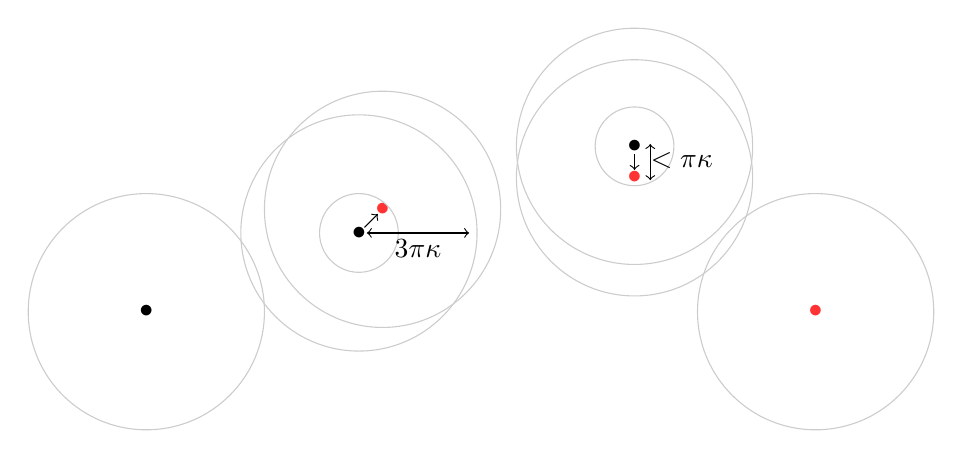
\begin{tikzpicture}
	% Pair 1
       	\draw[black] (0,0) node {$\bullet$} ;
	\draw[red!80] (.3,.3) node {$\bullet$} ; 
	\draw[->] 	(.07,.07)    	-- 	(.24,.24);
	\draw[black!20] (0,0) circle (1.5);
	\draw[black!20] (0,0) circle (0.5);
	\draw[black!20] (.3,.3) circle (1.5);
	\draw[<->]	(0.1,0)    	-- 	(1.4,0);
	\draw (0.75,-0.2)  node {$3\pi \kappa$};
	% Pair 2
	\draw[black] (3.5,1.1) node {$\bullet$} ;
	\draw[red!80] (3.5,0.7) node {$\bullet$} ; 
	\draw[->] 	(3.5,1.0)    	-- 	(3.5,0.8);
	\draw[black!20] (3.5,1.1) circle (1.5);
	\draw[black!20] (3.5,1.1) circle (0.5);
	\draw[black!20] (3.5,.7) circle (1.5);
	\draw[<->] 	(3.7,1.13)    	-- 	(3.7,0.67);
	\draw (4.1,0.92)  node {$<\pi \kappa$};
	% single black
	\draw[black] (-2.7,-1) node {$\bullet$} ;
	\draw[black!20] (-2.7,-1) circle (1.5);
	% single red
	\draw[red!80] (5.8,-1) node {$\bullet$} ;
	\draw[black!20] (5.8,-1) circle (1.5);
\end{tikzpicture}
        }
\caption{Configuration in dimension $2$ satisfying hypotheses of \thref{pairsdiracs}. The initial $\rho_0$ and final $\rho_1$ measures are composed of the black and red Dirac measures, respectively. At least 1 couple of spheres of radius $3\pi \kappa$ do not intersect for each pair of systems. We show that in that case, the geodesic is the sum of two travelling Dirac solutions (for the pairs), an on-place decreasing Dirac measure (single black) and an on place increasing Dirac measure (single red).}
\label{fig: matchingdiracs}
\end{figure}

\begin{proof}
Again we choose $\kappa=1$ without loss of generality. As for now, assume that all masses $h^i_0, h^i_1$ are strictly positive, the case of vanishing masses, i.e.\ ``single'' Dirac measures, will be fixed at the end of the proof. We aim at building an optimality certificate $\varphi \in C^1([0,1]\times \Om)$ for the candidate geodesic of the Theorem. Hence $\varphi $ should satisfy, for all $(t,x)\in [0,1]\times \Om$,
\[
\D_t \varphi +\frac12 \left( |\nabla \varphi| ^2 +  \varphi^2 \right) \leq 0
\]
and for all $t\in [0,1]$, for all $i\in \{ 1, \dots , N \}$ :
\[
\quad 
\begin{cases}
\nabla \varphi(x^i(t),t) = (x^i)'(t) \\
\varphi(x^i(t),t)=(h^i)'(t)/h^i(t) \\
\D_t \varphi +\frac12 \left( |\nabla \varphi |^2 + \varphi^2 \right) = 0 \quad  \text{for points of the form $(t,x^i(t))$}.
\end{cases}
\]

We introduce for $i\in \{1,\dots N\}$, the certificates $\varphi^i$ for the geodesics between each couple of Dirac measures $(h^i_0 \delta_{x^i_0}, h^i_1 \delta_{x^i_1})$ as defined in equation \eqref{certifddim}. The three parameters describing $\varphi^i$ are denoted $t^i_1, t^i_2$ and $\theta^i$. As $\theta^i$ is only defined up to translations, we decide from now on that $\theta^i$ is the unique such translation satisfying $\max\{ \vert x^i_0-\theta^i \vert, \vert x^i_1-\theta^i \vert \}< \pi$, which exists under our assumption that $|x_0^i - x_1^i|<\pi$. Thus, from the hypotheses in the Theorem, we have that $\min_{i \neq j}\{\vert \theta^i- \theta^j \vert \} > 4 \pi$. Now consider the \emph{binding} functions, defined for $i \in \{1,\dots,N \}$ by
\[
\varphi^i_b(t,x)=-\frac{1}{t-t^i_2} \cos(\vert x-\theta^i \vert ) + \frac{1}{t-t^i_2}. 
\]
Each $\varphi^i_b$ is in phase with $\varphi^i$ and satisfies 
\[
\varphi^i_b(t,\pi u + \theta^i)=\frac{2}{t-t_2^i}=\varphi^i(t,\pi u+ \theta^i) 
\quad \text{ and } \quad
\varphi^i_b(t,2\pi u+ \theta^i)=0
\]
for all $u\in \R^d$, $\vert u \vert = 1$ and $t\in[0,1]$. Also they are solutions to the equation $\D_t \varphi^i_b +\frac12 \left( (\nabla \varphi^i_b )^2 + (\varphi^i_b)^2 \right) = 0$. Now, as the constant zero function is a solution of this p.d.e too, we introduce
\begin{equation*}
\varphi(t,x)=
\begin{cases}
\varphi^i (t,x) & \text{if }  \vert x - \theta^i \vert \leq \pi \\
\varphi^i_b (t,x) & \text{if }  \vert x - \theta^i \vert \leq 2\pi  \text{ and } \vert x - \theta^i \vert > \pi\\
0 & \text{ otherwise.}
\end{cases}
\end{equation*}
Under the hypotheses of the Theorem, only one condition is met at a time so this function is well defined. It belongs to $C^1([0,1]\times \Om)$ because the bindings are located where the gradients vanish, on the extrema of cosines. See Figure \ref{figure certificate} to picture how the bindings are performed between the $\varphi^i$s. By construction, all hypotheses are fulfilled so that $\varphi$ be an optimality and uniqueness certificate.

Now if one or more of the $h^i_0$ or $h^i_1$ vanish, the same reasoning as in the proof of \thref{2diracs} allows to compute the distance between $\rho_0$ and $\rho_1$ (by an upper and lower bound, making the mass of vanishing Dirac measures tend to zero), and all that remains is to see that replacing the travelling Dirac solution by a Hellinger geodesic for single Dirac measures reaches that cost. 
\end{proof}

\begin{figure}%[ht]
\centering
 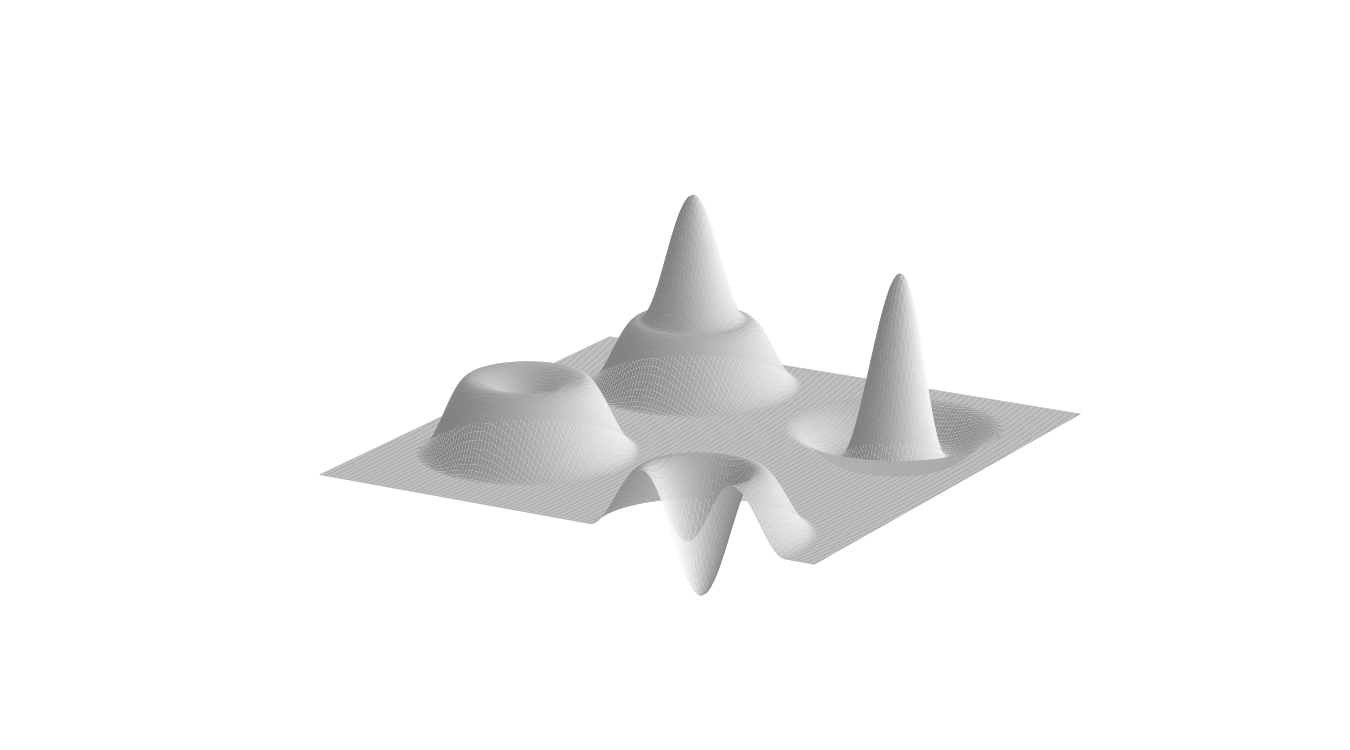
\includegraphics[trim=3cm 3cm 3cm 3cm, width=.7\linewidth]{images/certificate_dec2}%  ,clip,trim=15cm 10cm 15cm 15cm
 \caption{Example of an optimality certificate for $4$ pairs of Dirac measures, in the case $d=2$ at fixed $t$. The centers of the bumps are the $\theta^i$s. At the position $(t,x_i(t))$ of a travelling Dirac solution, the gradient gives its speed and the height gives its rate of growth.} 
 \label{figure certificate}
\end{figure}

%%%%%%%%%%%%%%%%%%%%%%%%%%%%%
